% =============================================================================
%  CHAPTER 6: Figures and Floats
% =============================================================================

\chapter{Figures \& Images}

\section{Including Images (graphicx)}

\begin{lstlisting}[language={[LaTeX]TeX}, caption=Including images]
\usepackage{graphicx}

% Basic image:
\includegraphics{filename}

% With options:
\includegraphics[width=5cm]{filename}
\includegraphics[height=3cm]{filename}
\includegraphics[scale=0.5]{filename}
\includegraphics[width=\textwidth]{filename}
\includegraphics[width=0.8\textwidth]{filename}
\includegraphics[angle=90]{filename}       % Rotate 90 degrees
\includegraphics[clip=true, trim=1cm 2cm 1cm 2cm]{filename} % Crop

% Supported formats: PDF, PNG, JPG, EPS
\end{lstlisting}

\begin{figure}[H]
    \centering
    \includegraphics[width=0.4\textwidth]{example-image-a}
    \caption{Example image A using \texttt{example-image-a}}
    \label{fig:exampleA}
\end{figure}

% ------------------------------------------------------------------
\section{Figure Environment (Float)}

\begin{lstlisting}[language={[LaTeX]TeX}, caption=Figure float]
\begin{figure}[htbp]
    \centering
    \includegraphics[width=0.6\textwidth]{myimage}
    \caption{Description of the image.}
    \label{fig:mylabel}
\end{figure}

% Placement specifiers:
% h = here, t = top, b = bottom, p = float page
% ! = override LaTeX rules, H = exactly HERE (float package)
\end{lstlisting}

\subsection{Referencing Figures}

As seen in Figure~\ref{fig:exampleA}, we can reference images by their label.

\begin{lstlisting}[language={[LaTeX]TeX}, caption=Referencing figures]
% In text:
As shown in Figure~\ref{fig:mylabel} ...

% The ~ prevents a line break between "Figure" and the number.
\end{lstlisting}

% ------------------------------------------------------------------
\section{Subfigures (subcaption package)}

\begin{lstlisting}[language={[LaTeX]TeX}, caption=Subfigures]
\usepackage{subcaption}

\begin{figure}[htbp]
    \centering
    \begin{subfigure}[b]{0.45\textwidth}
        \includegraphics[width=\textwidth]{image1}
        \caption{First subfigure}
        \label{fig:sub1}
    \end{subfigure}
    \hfill
    \begin{subfigure}[b]{0.45\textwidth}
        \includegraphics[width=\textwidth]{image2}
        \caption{Second subfigure}
        \label{fig:sub2}
    \end{subfigure}
    \caption{Overall caption for both subfigures}
    \label{fig:combined}
\end{figure}
\end{lstlisting}

\begin{figure}[H]
    \centering
    \begin{subfigure}[b]{0.4\textwidth}
        \includegraphics[width=\textwidth]{example-image-a}
        \caption{Subfigure A}
        \label{fig:subA}
    \end{subfigure}
    \hfill
    \begin{subfigure}[b]{0.4\textwidth}
        \includegraphics[width=\textwidth]{example-image-b}
        \caption{Subfigure B}
        \label{fig:subB}
    \end{subfigure}
    \caption{Two subfigures side by side}
    \label{fig:subfigures}
\end{figure}

% ------------------------------------------------------------------
\section{Image Size Options}

\begin{table}[H]
\centering
\begin{tabular}{ll}
\toprule
\textbf{Option} & \textbf{Description} \\
\midrule
\verb|width=5cm|         & Set exact width \\
\verb|height=3cm|        & Set exact height \\
\verb|width=\textwidth|  & Scale to text width \\
\verb|width=0.5\textwidth| & Half text width \\
\verb|scale=0.5|         & Scale to 50\% \\
\verb|angle=45|          & Rotate 45 degrees \\
\verb|clip=true|         & Clip to bounding box \\
\verb|trim=l b r t|      & Trim from left, bottom, right, top \\
\verb|keepaspectratio|   & Maintain proportions \\
\bottomrule
\end{tabular}
\caption{Image sizing options}
\end{table}

% ------------------------------------------------------------------
\section{Wrapping Text Around Images}

\begin{lstlisting}[language={[LaTeX]TeX}, caption=wrapfig]
\usepackage{wrapfig}

\begin{wrapfigure}{r}{0.4\textwidth}
    \centering
    \includegraphics[width=\linewidth]{image}
    \caption{Wrapped figure}
\end{wrapfigure}

This text will wrap around the figure on the left side.
% {r} = right side, {l} = left side, {R} = right (allows floating)
\end{lstlisting}

% ------------------------------------------------------------------
\section{Drawing Simple Graphics with TikZ (Preview)}

TikZ can also be used inside figure environments:

\begin{figure}[H]
    \centering
    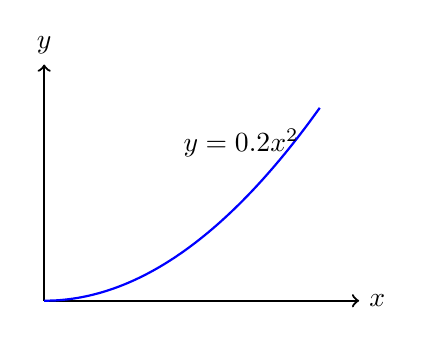
\begin{tikzpicture}
        \draw[thick, ->] (0,0) -- (4,0) node[right] {$x$};
        \draw[thick, ->] (0,0) -- (0,3) node[above] {$y$};
        \draw[blue, thick, domain=0:3.5, smooth, variable=\x] plot ({\x}, {0.2*\x*\x});
        \node at (2.5, 2) {$y = 0.2x^2$};
    \end{tikzpicture}
    \caption{A simple plot drawn with TikZ}
    \label{fig:tikzplot}
\end{figure}
